% 图 14.1 —— 由 `checks/emit_hand.py` 自动拼出（probe 精测 + prims2 图元分解）
%%
% ⚠ 这是**稿子不是成品**：跑 `checks/checkhand.py 14.1` 看指标 + 看叠合图。
%%
%% ⚠ 待核：
%   · 本图 probe 报出阴影族 1 个 —— **本脚本不生成阴影**（要照原书手写）；prims2 的 strokes 里可能含阴影线，核对时留意别画重
%   · 可疑字形 1 项（空心圈 ⊙ 常被认成字母 o）—— 见文件末
%%
\documentclass[12pt]{standalone}
\usepackage{fontspec}
\setsansfont{Arial}
\newfontfamily\mfallback{DejaVu Sans}
\usepackage{tikz}
\begin{document}
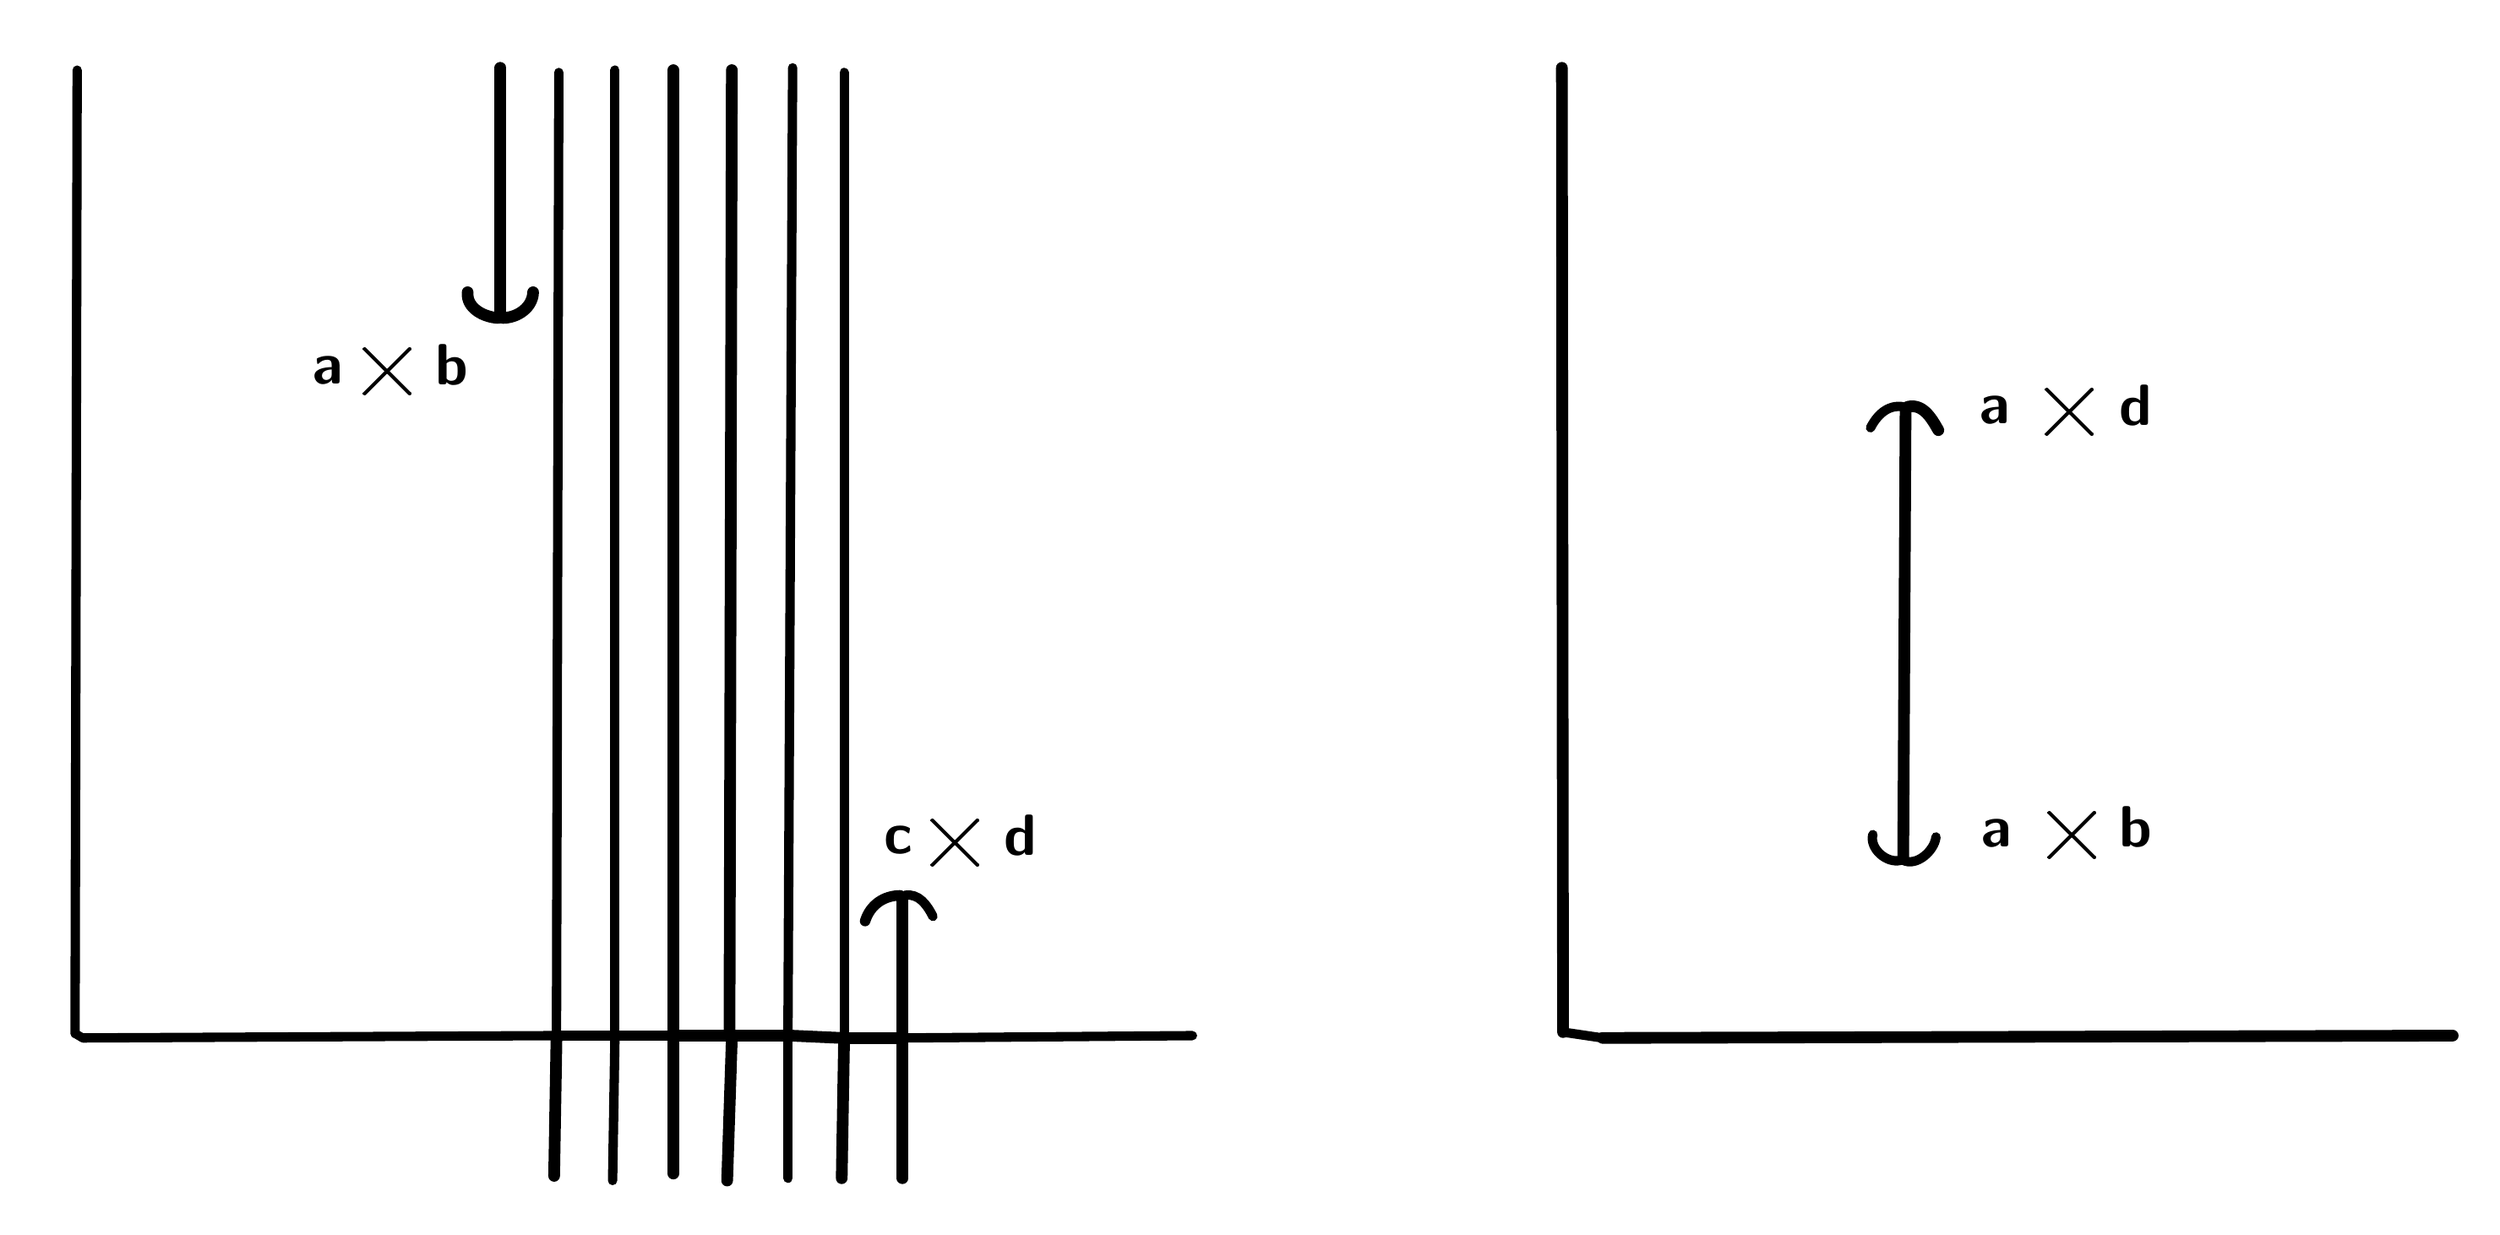
\begin{tikzpicture}[x=1pt, y=-1pt, line width=5.0pt, line cap=round, line join=round]

  %% ════ 直线段（prims2 的 strokes）════
  \draw[line width=5.0pt] (804.0,357.0) -- (805.0,165.0);
  \draw[line width=4.0pt] (327.0,494.0) -- (327.0,434.0);
  \draw[line width=5.0pt] (301.0,495.0) -- (303.0,434.0);
  \draw[line width=4.0pt] (327.0,432.0) -- (329.0,19.0);
  \draw[line width=4.0pt] (500.0,433.0) -- (377.0,434.0);
  \draw[line width=5.0pt] (326.0,433.0) -- (304.0,433.0);
  \draw[line width=5.0pt] (303.0,20.0) -- (302.0,432.0);
  \draw[line width=5.0pt] (301.0,433.0) -- (279.0,433.0);
  \draw[line width=5.0pt] (658.0,19.0) -- (658.5,431.5);
  \draw[line width=4.0pt] (658.5,431.5) -- (675.4,434.0);
  \draw[line width=5.0pt] (675.4,434.0) -- (1039.0,433.0);
  \draw[line width=5.0pt] (278.0,20.0) -- (278.0,432.0);
  \draw[line width=5.0pt] (328.0,433.0) -- (350.0,434.0);
  \draw[line width=5.0pt] (350.0,494.0) -- (351.0,435.0);
  \draw[line width=5.0pt] (375.0,434.0) -- (352.0,434.0);
  \draw[line width=5.0pt] (376.0,433.0) -- (376.0,374.0);
  \draw[line width=4.0pt] (252.0,433.0) -- (229.0,433.0);
  \draw[line width=4.0pt] (228.0,432.0) -- (229.0,21.0);
  \draw[line width=4.0pt] (227.0,433.0) -- (25.4,434.0);
  \draw[line width=3.8pt] (25.4,434.0) -- (22.1,432.1);
  \draw[line width=4.0pt] (22.1,432.1) -- (23.0,20.0);
  \draw[line width=4.0pt] (254.0,433.0) -- (277.0,433.0);
  \draw[line width=5.0pt] (228.0,434.0) -- (227.0,493.0);
  \draw[line width=4.0pt] (252.0,495.0) -- (253.0,434.0);
  \draw[line width=4.0pt] (351.0,21.0) -- (351.0,433.0);
  \draw[line width=5.0pt] (278.0,434.0) -- (278.0,492.0);
  \draw[line width=4.0pt] (253.0,432.0) -- (253.0,20.0);
  \draw[line width=5.0pt] (376.0,494.0) -- (376.0,435.0);
  \draw[line width=5.0pt] (204.0,125.0) -- (204.0,19.0);

  %% ════ 曲线（prims2 的 curves —— 三段式，坐标同为 (y,x)）════
  \draw[line width=5.0pt] (190.0,115.0) .. controls (189.4,122.0) and (197.2,125.7) .. (203.0,126.0);
  \draw[line width=4.0pt] (803.0,358.0) .. controls (796.7,359.6) and (789.4,352.7) .. (791.0,347.0);
  \draw[line width=4.5pt] (375.0,373.0) .. controls (368.0,373.1) and (362.2,377.0) .. (360.0,384.0);
  \draw[line width=4.0pt] (377.0,373.0) .. controls (383.0,371.9) and (386.7,377.4) .. (389.0,382.0);
  \draw[line width=4.0pt] (804.0,164.0) .. controls (797.3,162.9) and (792.7,167.7) .. (790.0,173.0);
  \draw[line width=5.0pt] (806.0,164.0) .. controls (812.6,162.5) and (816.3,169.3) .. (819.0,174.0);
  \draw[line width=5.0pt] (205.0,126.0) .. controls (211.1,126.0) and (217.8,121.7) .. (218.0,115.0);
  \draw[line width=4.0pt] (818.0,348.0) .. controls (817.4,353.9) and (809.7,360.8) .. (804.0,358.0);

  %% ════ 标签（probe 直接给的 \node 行）════
  %% ⚠ 全部补了 fill=white：文字在最上层，否则与曲线交叉干扰
     \node[anchor=center,inner sep=0pt,fill=white,font=\fontsize{30.7}{38.3}\selectfont] at (183.3,145.9) {\textsf{\textbf{\textit{b}}}};   % box(184,142,17,23)
     \node[anchor=center,inner sep=0pt,fill=white,font=\fontsize{33.8}{42.2}\selectfont] at (155.6,149.0) {\textsf{\textbf{×}}};   % box(158,146,15,16)
     \node[anchor=center,inner sep=0pt,fill=white,font=\fontsize{32.0}{40.0}\selectfont] at (130.5,148.5) {\textsf{\textbf{\textit{a}}}};   % box(133,147,16,17)
     \node[anchor=center,inner sep=0pt,fill=white,font=\fontsize{29.3}{36.6}\selectfont] at (903.5,163.4) {\textsf{\textbf{\textit{d}}}};   % box(893,160,18,21)
     \node[anchor=center,inner sep=0pt,fill=white,font=\fontsize{34.9}{43.6}\selectfont] at (875.2,166.5) {\textsf{\textbf{×}}};   % box(866,163,16,16)
     \node[anchor=center,inner sep=0pt,fill=white,font=\fontsize{32.0}{40.0}\selectfont] at (843.5,165.5) {\textsf{\textbf{\textit{a}}}};   % box(835,164,16,17)
     \node[anchor=center,inner sep=0pt,fill=white,font=\fontsize{30.0}{37.6}\selectfont] at (903.6,343.7) {\textsf{\textbf{\textit{b}}}};   % box(893,337,17,22)
     \node[anchor=center,inner sep=0pt,fill=white,font=\fontsize{30.0}{37.6}\selectfont] at (426.4,347.2) {\textsf{\textbf{\textit{d}}}};   % box(424,340,18,22)
     \node[anchor=center,inner sep=0pt,fill=white,font=\fontsize{33.8}{42.2}\selectfont] at (876.2,347.4) {\textsf{\textbf{×}}};   % box(867,341,15,16)
     \node[anchor=center,inner sep=0pt,fill=white,font=\fontsize{33.0}{41.2}\selectfont] at (844.0,346.6) {\textsf{\textbf{\textit{a}}}};   % box(835,342,17,17)
     \node[anchor=center,inner sep=0pt,fill=white,font=\fontsize{31.4}{39.3}\selectfont] at (374.3,349.6) {\textsf{\textbf{\textit{c}}}};   % box(374,345,16,17)
     \node[anchor=center,inner sep=0pt,fill=white,font=\fontsize{33.8}{42.2}\selectfont] at (398.5,350.8) {\textsf{\textbf{×}}};   % box(397,345,15,16)

  % 钉死画布：否则超出的图元/控制点会把页面撑大，1:1 回比就失准
  \pgfresetboundingbox
  \path[use as bounding box] (0,0) rectangle (1049,508);
\end{tikzpicture}
\end{document}

% ⚠ 待核清单（probe 拿不准，人眼过一遍）：
%   · 未识别/跳过：⑤ 跳过/未识别的字形
